%!TEX root = guide2.0.tex

% \section{Summary}\label{sec:PyMCObjects}
Bayesian inference begins with specification of a probability model relating unknown variables to data. PyMC provides three basic building blocks for Bayesian probability models: \texttt{Stochastic}, \texttt{Deterministic} and \texttt{Potential}. 

A \texttt{Stochastic} object represents a variable whose value is not completely determined by its parents, and a \texttt{Deterministic} object represents a variable that is determined by its parents. \texttt{Stochastic} and \texttt{Deterministic} are subclasses of \texttt{Variable}. The third basic class, representing `factor potentials' (\cite{dawidmarkov,jordangraphical}), represents a arbitrary log-probability terms. \texttt{Potential} and \texttt{Variable} are subclasses of \texttt{Node}.

% PyMC also provides container classes for variables to make it easier to program of certain dependency situations, such as when a variable is defined by its dependence on an entire Markov chain.

\medskip
PyMC probability models are simply linked groups of \texttt{Stochastic}, \texttt{Deterministic} and \texttt{Potential} objects. These objects have very limited awareness of the models in which they are embedded and no methods for updating their values in fitting algorithms. Objects responsible for fitting probability models are described in chapter \ref{chap:modelfitting}.
 

\hypertarget{stochastic}{}
\section*{The \texttt{Stochastic} class} \label{stochastic}
\pdfbookmark[0]{The Stochastic class}{stochastic}

A stochastic variable has the following major attributes: 
\begin{description}
    \item[\texttt{value}:] The variable's current value.
    \item[\texttt{logp}:] The log-probability of the variable's current value given the values of its parents.
\end{description}
A stochastic variable can optionally be endowed with a method called \texttt{\bfseries random}, which draws a value for the variable given the values of its parents. Note that the \texttt{random} method does not provide a Gibbs sample unless the variable has no children.

A stochastic variable has the following additional attributes:
\begin{description}
    \item[\texttt{parents}:] A dictionary containing the variable's parents. The keys of the dictionary correspond to the names assigned to the variable's parents by the variable, and the values correspond to the actual parents. For example, the keys of $s$'s parents dictionary in model (\ref{disastermodel}) would be \texttt{'t_l'} and \texttt{'t_h'}. Thanks to Python's dynamic typing, the actual parents (the values of the dictionary) may be of any class or type.
    \item[\texttt{children}:] A set containing the variable's children. This set is produced automatically; the user doesn't need to worry about filling it.
    \item[\texttt{extended_parents}:] A set containing all the stochastic variables on which the variable depends either directly or via a sequence of deterministic variables. If the value of any of these variables changes, the variable will need to recompute its log-probability. This set is produced automatically.
    \item[\texttt{extended_children}:] A set containing all the stochastic variables and potentials that depend on the variable either directly or via a sequence of deterministic variables. If the variable's value changes, all of these variables will need to recompute their log-probabilities. This set is produced automatically.
    \item[\texttt{coparents}:] A set containing all the stochastic variables that share extended children with the variable.
    \item[\texttt{moral_neighbors}:] A set containing the union of the variable's extended parents, extended children and coparents, with potentials removed.
    \item[\texttt{markov_blanket}:] A set containing self and self's moral neighbors.
    \item[\texttt{isdata}:] A boolean indicating whether the variable's value has been observed (is fixed).
    \item[\texttt{dtype}:] A NumPy dtype object (such as \texttt{numpy.int}) or \texttt{None}. If it is not None, this attribute signals the type of the variable's value to fitting methods.
    \item[\texttt{__name__}:] The name of the variable, should be unique.
    \item[\texttt{__doc__}:] The docstring of the variable.
\end{description}

\subsection{Creation of stochastic variables}
There are four ways to create stochastic variables, called the `automatic', `short', `long' and `direct' interfaces.

\begin{description}    
    \item[Automatic] Stochastic variables with standard distributions (see chapter \ref{chap:distributions} ) can be created in a single line using special subclasses of \texttt{Stochastic}. Uniformly-distributed discrete variable $s$ in (\ref{disastermodel}) could be created using the automatic interface as follows:
    \begin{verbatim}
        s = DiscreteUniform('s', 1851, 1962, value=1900)
    \end{verbatim}

    In addition to the classes in chapter \ref{chap:distributions}, \texttt{scipy.stats.distributions}' random variable classes are wrapped as \texttt{Stochastic} subclasses if SciPy is installed. These distributions are in the submodule \texttt{pymc.SciPyDistributions}

    You can use the class factory \texttt{stochastic_from_dist} to produce \texttt{Stochastic} subclasses from probability distributions not included with PyMC.%  These classes' init methods take the following arguments:
    % \begin{description}
    %     \item[\texttt{name}:] The name of the variable.
    %     \item[\texttt{value}:] An initial value for the variable.
    %     \item[\texttt{parents}:] Keyword arguments specifying the parents of the variable.
    %     \item[\texttt{isdata} (optional)]
    %     \item[\texttt{doc} (optional):] The docstring of the variable.
    %     \item[\texttt{verbose} (optional):] An integer from 0 to 3.
    %     \item[\texttt{trace} (optional):] A boolean indicating whether a trace should be kept for this variable in Monte Carlo fitting methods.
    %     \item[\texttt{cache_depth}:] See section \ref{sec:caching}. 
    % \end{description}
    
    
    \item[Short] Uniformly-distributed discrete stochastic variable $s$ in (\ref{disastermodel}) could be created as follows:
    \begin{verbatim}
@stochastic(dtype=int)
def s(value=1900, t_l=1851, t_h=1962):
    """The switchpoint for the rate of disaster occurrence."""
    if value > t_h or value < t_l:
        return -Inf
    else:
        return -log(t_h - t_l + 1) 
    \end{verbatim}
    The \texttt{Stochastic} object produced by the decorator \texttt{stochastic} will evaluate its log-probability using the function \texttt{s}. The \texttt{value} argument, which is required, provides an initial value for the variable. The names of the function \texttt{s}'s other arguments will become the keys of the stochastic variable \texttt{s}'s \texttt{parents} dictionary. The values of these arguments will become the values of the dictionary.

Stochastic variables may be valued as any object and their parents may be any objects as long as their log-probability functions return a real number (NumPy \texttt{float}). PyMC and SciPy both provide fast implementations of several standard probability distributions that may be helpful for creating custom stochastic variables.

    The decorator \texttt{stochastic} can take several arguments: 
    \begin{itemize}
        \item A flag called \texttt{trace}, which signals to \texttt{MCMC} instances whether an MCMC trace should be kept for the stochastic variable. \texttt{@stochastic(trace = False)} would turn tracing off.
        \item A flag called \texttt{plot}, which signals to \texttt{MCMC} instances whether summary plots should be produced for this variable.
        \item An integer-valued argument called \texttt{verbose} that controls the amount of output the variable prints to the screen. The default is $0$, no output; the maximum value is 3. 
        \item A NumPy datatype called \texttt{dtype}. Decorating a log-probability function with \texttt{@stochastic(dtype=int)} would produce a discrete random variable. Such a variable will cast its value to either an integer or an array of integers. The default dtype is \texttt{float}.
    \end{itemize} 
    

    \item[Long] The long interface allows you to specify a \texttt{random} method for sampling the stochastic variable's value conditional on its parents.
    \begin{verbatim}
@stochastic(dtype=int)
def s(value=1900, t_l=1851, t_h=1962):
    """The switchpoint for the rate of disaster occurrence."""

    def logp(value, t_l, t_h):
        if value > t_h or value < t_l:
            return -Inf
        else:
            return -log(t_h - t_l + 1) 
            
    def random(t_l, t_h):
        return round( (t_l - t_h) * random() ) + t_l

    rseed = 1.
    \end{verbatim}
The stochastic variable again gets its name, docstring and parents from function $s$, but in this case it will evaluate its log-probability using the \texttt{logp} function. The \texttt{random} function will be used when \texttt{s.random()} is called. Note that it doesn't take a \texttt{value} argument, because it provides a new value. \texttt{rseed} provides a seed for the RNG. The \texttt{value} argument is optional if a \texttt{random} method is provided; if no initial value is provided, it will be drawn using the \texttt{random} method.

    \item[Direct] It's possible to instantiate \texttt{Stochastic} directly:
\begin{verbatim}
def s_logp(value, t_l, t_h):
    if value > t_h or value < t_l:
        return -Inf
    else:
        return -log(t_h - t_l + 1) 

def s_rand(t_l, t_h):
    return round( (t_l - t_h) * random() ) + t_l

s = Stochastic( logp = s_logp, 
                doc = 'The switchpoint for the rate of disaster occurrence.',
                name = 's', 
                parents = {'t_l': 1851, 't_h': 1962},
                random = s_rand,                 
                trace = True,                 
                value = 1900,
                dtype=int,
                rseed = 1., 
                isdata = False,
                cache_depth = 2,
                plot=True,
                verbose = 0)
\end{verbatim}
\end{description}

\hypertarget{sub:warning}{}
\subsection*{Don't update stochastic variables' values in-place} \label{sub:warning}
\pdfbookmark[0]{Don't update stochastic variables' values in-place}{sub:warning}

\texttt{Stochastic} objects' values should not be updated in-place. This would confuse PyMC's caching scheme and corrupt the `last value' attribute, which is used for rejecting jumps. The only way a stochastic variable's value should be updated is using statements of the following form:
\begin{verbatim}
    A.value = new_value
\end{verbatim}
The following are in-place updates and should \emph{not} be used:
\begin{itemize}
    \item \texttt{A.value += 3}
    \item \texttt{A.value[2,1] = 5}
    \item \texttt{A.value.attribute = new_attribute_value}.
\end{itemize}

This restriction becomes onerous if a step method proposes values for the elements of an array-valued variable separately. In this case, it may be preferable to partition the variable into several variables stored in an array or list.

\hypertarget{data}{}
\section*{Data} \label{data}
\pdfbookmark[0]{Data}{data}

Although the data $D$ is represented by a random variable in the model, we have fixed its value by observing it. Such variables are represented by \texttt{Stochastic} objects whose \texttt{isdata} attribute is set to \texttt{True}. If a stochastic variable's \texttt{isdata} flag is \texttt{True}, its value cannot be changed.

\subsection*{Declaring stochastic variables to be data}

In the short and long interfaces, a \texttt{Stochastic} object's \texttt{isdata} flag can be set to true by stacking a \texttt{@data} decorator on top of the \texttt{@stochastic} decorator:
\begin{verbatim}
@data
@stochastic(dtype=int)
def D(value = count_array, switchpoint = s, early_rate = e, late_rate = l):
    """The observed annual disaster counts."""
    logp = sum(-value[:switchpoint]) + early_rate * log(value[:switchpoint]) \
            - gammaln(early_rate))
    logp += sum(-value[switchpoint:] + late_rate * log(value[switchpoint:]) \
            - gammaln(late_rate))
    return logp
\end{verbatim}
In the automatic and direct interfaces, the \texttt{isdata} argument can be simply set to \texttt{True}.


\hypertarget{deterministic}{}
\section*{The \texttt{Deterministic} class} \label{deterministic}
\pdfbookmark[0]{The Deterministic class}{deterministic}

The \texttt{Deterministic} class represents variables whose values are fully determined by the values of their parents. In model (\ref{disastermodel}), $r$ can be represented as a deterministic variable. Recall that $r$ was defined by
\begin{eqnarray*}
    r_t=\left\{\begin{array}{ll}
        e & t\le s\\ l & t>s
        \end{array}\right.,
\end{eqnarray*}
so $r$'s value can be computed from the values of its parents $e$, $l$ and $s$.

A deterministic variable's most important attribute is \texttt{\bfseries value}, which gives the current value of the variable given the values of its parents. Like \texttt{Stochastic}'s \texttt{logp} attribute, this attribute is computed on-demand and cached for efficiency.

A Deterministic variable has the following additional attributes:
\begin{description}
    \item[\texttt{parents}:] A dictionary containing the variable's parents. The keys of the dictionary correspond to the names assigned to the variable's parents by the variable, and the values correspond to the actual parents. Thanks to Python's dynamic typing, parents may be of any class or type.
    \item[\texttt{children}:] A set containing the variable's children, which must be nodes. This set is produced automatically; the user doesn't need to worry about filling it.
    \item[\texttt{__name__}:] The name of the variable, should be unique.
    \item[\texttt{__doc__}:] The docstring of the variable.
\end{description}
Deterministic variables have no methods.


\subsection*{Creation of deterministic variables}
Deterministic variables are less complicated than stochastic variables, and there are only three ways to create them:
\begin{description}
   \item[Automatic] A handful of functions have been wrapped in Deterministic objects. These are brief enough to list:
   \begin{description}
      \item[\texttt{LinearCombination}:] Has two parents $x$ and $y$, both of which must be iterables. Valued as
      \[
      \sum_i x_i^T y_i.
      \]
      \item[\texttt{Index}:] Has three parents $x$, $y$ and \texttt{index}. $x$ and $y$ must be iterables, \texttt{index} must be valued as an integer. Valued as
      \[
      x_{\mathtt{index}}^T y_{\mathtt{index}}.
      \]
      \texttt{Index} is useful for implementing `dynamic' models, in which the parent-child connections change.
      \item[\texttt{Lambda}:] Converts an anonymous function to a \texttt{Deterministic} instance on a single line.
      \item[\texttt{CompletedDirichlet}:] PyMC represents Dirichlet variables of length $k$ by the first $k-1$ elements; since they must sum to 1, the $k$'th element is determined by the others. \texttt{CompletedDirichlet} appends the $k$'th element to the value of its parent $D$.      
      \item[\texttt{Logit}, \texttt{InvLogit}, \texttt{StukelLogit}, \texttt{StukelInvLogit}:] Various common link functions for generalized linear models.
   \end{description}
   It's a good idea to use these classes when feasible, because certain fitting methods (Gibbs step methods in particular) know how to take them into account.
    \item[Decorator] A deterministic variable can be created via a decorator in a way very similar to \texttt{Stochastic}'s short interface:
\begin{verbatim}
@deterministic
def r(switchpoint = s, early_rate = e, late_rate = l):
    """The rate of disaster occurrence."""
    value = zeros(N)
    value[:switchpoint] = early_rate
    value[switchpoint:] = late_rate
    return value
\end{verbatim}
The function supplied should return a new value (which may be any object) for the variable. Arguments' keys and values are converted into a parent dictionary as with \texttt{Stochastic}'s short interface. The function's \texttt{__name__} is passed on to the variable. The \texttt{deterministic} decorator can take \texttt{trace} and \texttt{verbose} arguments, like the \texttt{stochastic} decorator.
    \item[Direct] The same variable could be created directly as follows:
\begin{verbatim}
def r_eval(switchpoint = s, early_rate = e, late_rate = l):
    value = zeros(N)
    value[:switchpoint] = early_rate
    value[switchpoint:] = late_rate
    return value

r = Deterministic(  eval = r_eval, 
                    name = 'r',
                    parents = {'switchpoint': s, 'early_rate': e, 'late_rate': l}),
                    doc = 'The rate of disaster occurrence.',
                    trace = True,
                    verbose = 0,
                    cache_depth = 2)
\end{verbatim}
The \texttt{trace} flag signals to \texttt{Model} whether to keep a trace for the variable, as with stochastic variables.
\end{description}

Note that deterministic variables have no \texttt{isdata} flag. If a deterministic variable's value were known, its parents would be restricted to the inverse image of that value under the deterministic variable's evaluation function. This usage would be extremely difficult to support in general, but it can be implemented for particular applications at the \texttt{StepMethod} level.

\hypertarget{container}{}
\section*{Containers} \label{container}
\pdfbookmark[0]{Containers}{container}

In the following situation, it would be inconvenient to assign a unique label to each parent of $y$:
\begin{eqnarray*}
    x_0 \sim \textup N(0,\tau_x)\\
    x_{i+1}|x_i\sim\textup{N}(x_i, \tau_x),& i=0\ldots N-2\\
    y|x \sim \textup N\left(\sum_{i=0}^{N-1}x_i^2,\tau_y\right).
\end{eqnarray*}
$y$ depends on every element of the Markov chain $x$, but we wouldn't want to manually enter $N$ parent labels \texttt{'x_0'}, \texttt{'x_1'}, etc.

This situation can be handled in the natural way:
\begin{verbatim}
x_0 = Normal('x_0', mu=0, tau=1)

x = [x_0]
last_x = x_0

for i in range(1,N):          
   x_now = Normal('x_%i'%i, mu=last_x, tau=1)        
   last_x = x_now 
   x.append(x_now)

@data
@stochastic
def y(value = 1, mu = x, tau = 100):
    mu_sum = 0
    for i in range(N):
        mu_sum += mu[i] ** 2
    return normal_like(value, mu_sum, tau)
\end{verbatim}
The list \texttt{x} is transparently wrapped in an appropriate container class by the function \texttt{Container}.

Containers, like variables, have an attribute called \texttt{value}. This attribute returns a copy of the (possibly nested) iterable that was passed into the container function, but with each variable inside replaced with \emph{its} value. 

Containers can currently be constructed from lists, tuples, dictionaries, NumPy arrays, modules, sets and any object with a \texttt{__dict__} attribute. Variables and non-variables can be freely mixed in these containers, and different types of containers can be nested. Containers attempt to behave like the objects they wrap. All containers are subclasses of \texttt{ContainerBase}. 

Nodes whose parents are containers make private shallow copies of those containers. This is done for technical reasons rather than to protect users from accidental misuse.

Containers have the following useful attributes in addition to \texttt{value}:
\begin{itemize}
    \item\texttt{variables}
    \item\texttt{stochastics}
    \item\texttt{potentials}
    \item\texttt{deterministics}
    \item\texttt{data_stochastics}
    \item\texttt{step_methods}.
\end{itemize}
Each of these attributes is a set containing all the objects of each type in a container, and within any containers in the container.


\hypertarget{potential}{}
\section*{The Potential class} \label{potential}
\pdfbookmark[0]{The Potential class}{potential}

% WE PROBABLY NEED TO GIVE A GOOD EXAMPLE OF WHERE A POTENTIAL IS DIFFERENT FROM A DETERMINISTIC;
% THIS PROBABLY WONT BE CLEAR TO EVERYONE. THE KEY DIFFERENCE IS THAT A POTENTIAL IS PART OF THE
% JOINT POSTERIOR, NO?
% 

The joint density corresponding to model (\ref{disastermodel}) can be written as follows:
\begin{eqnarray*}
    p(D,s,l,e) = p(D|s,l,e) p(s) p(l) p(e).
\end{eqnarray*}
Each factor in the joint distribution is a proper, normalized probability distribution for one of the variables conditional on its parents. Such factors are contributed by \texttt{Stochastic} objects.

In some cases, it's nice to be able to modify the joint density by incorporating terms that don't correspond to probabilities of variables conditional on parents, for example:
\begin{eqnarray*}
    p(x_0, x_2, \ldots x_{N-1}) \propto \prod_{i=0}^{N-2} \psi_i(x_i, x_{i+1}).
\end{eqnarray*}
Arbitrary factors such as $\psi$ are contributed by objects of class \texttt{Potential} (\cite{dawidmarkov} and \cite{jordangraphical} call these terms `factor potentials'). Bayesian hierarchical notation (cf model (\ref{disastermodel})) doesn't accomodate these potentials. They are most useful in cases where there is no natural dependence hierarchy, such as Markov random fields. They are also useful for expressing `soft data' \cite{christakos} 

% Even when there is a definite dependence hierarchy, potentials can provide a useful shorthand. Consider a new example: we have a dataset $t$ consisting of the days on which several marked animals were recaptured. We believe that the probability $S$ that an animal is not recaptured on any given day can be explained by a covariate vector $x$. We model this situation as follows:
% \begin{eqnarray*}
%     t_i|S_i \sim \textup{Geometric}(S_i), & i=1\ldots N\\
%     S_i = \textup{logit}^{-1}(\beta x_i), &i=1\ldots N\\
%     \beta\sim \textup{N}(\mu_\beta, V_\beta).
% \end{eqnarray*}
% So far, so good. Now suppose we have some knowledge of other related experiments and we have a good idea of what $S$ will be before seeing the data. It's not obvious how to work this prior information in, because as we've written the model $S$ is completely determined by $\beta$. There are three options within the strict Bayesian hierarchical framework:
% \begin{itemize}
%     \item Work the prior information into the prior on $\beta$.
%     \item Incorporate the data from the previous experiments explicitly into the model.
%     \item Refactor the model so that $S$ is at the bottom of the hierarchy, and assign the prior directly.
% \end{itemize}
% 
% Factor potentials provide a convenient way to incorporate the prior information without the need for such major modifications. We can simply modify the joint distribution from
% \begin{eqnarray*}
%     p(t|S(x,\beta)) p(\beta)
% \end{eqnarray*}
% to
% \begin{eqnarray*}
%     \gamma(S,a,b) p(t|S(x,\beta)) p(\beta),
% \end{eqnarray*}
% where $\gamma$ expresses the prior information. It's a good idea to check the induced priors on $S$ and $\beta$ for sanity. This can be done in PyMC by fitting the model with the data $t$ commented out.

\bigskip
Potentials have one important attribute, \texttt{\bfseries logp}, which gives the log of their current probability or probability density value given the values of their parents. They have the following additional attributes:
\begin{description}
    \item[\texttt{parents}:] A dictionary containing the potential's parents. The keys of the dictionary correspond to the names assigned to the potential's parents by the potential, and the values correspond to the actual parents. Thanks to Python's dynamic typing, parents may be of any class or type.
    \item[\texttt{__name__}:] The name of the potential, should be unique.
    \item[\texttt{__doc__}:] The docstring of the potential.
\end{description}
Potentials have no methods. They have no \texttt{trace} attribute, because they are not variables. They cannot serve as parents of variables for the same reason, so they have no \texttt{children} attribute.


\subsection*{Creation of \texttt{Potentials}}
There are two ways to create potentials:
\begin{description}
    \item[Decorator] A potential can be created via a decorator in a way very similar to \texttt{Stochastic}'s short interface and \texttt{Deterministic}'s decorator interface:
\begin{verbatim}
@potential
def psi_i(x_lo = x[i], x_hi = x[i+1]):
    """A pair potential"""
    return -(xlo - xhi)**2
\end{verbatim}
The function supplied should return a NumPy \texttt{float}. Arguments' names and values are converted into a parent dictionary as with \texttt{Stochastic}'s medium interface. The function's \texttt{__name__} is passed on to the potential. The \texttt{potential} decorator can take \texttt{verbose} and \texttt{cache_depth} arguments like the \texttt{stochastic} decorator.
    \item[Direct] The same potential could be created directly as follows:
\begin{verbatim}
def psi_i_logp(x_lo = x[i], x_hi = x[i+1]):
    return -(xlo - xhi)**2
        
psi_i = Potential(  logp = psi_i_logp, 
                    name = 'psi_i',
                    parents = {'xlo': x[i], 'xhi': x[i+1]},
                    doc = 'A pair potential',
                    verbose = 0,
                    cache_depth = 2)
\end{verbatim}
\end{description}


\hypertarget{graphical}{}
\section*{Graphing models} \label{graphical}
\pdfbookmark[0]{Graphing models}{graphical}

The function \texttt{graph} draws graphical representations of \texttt{Model} (chapter \ref{chap:modelfitting}) instances using GraphViz via the Python package PyDot. See \cite{dawidmarkov} and \cite{jordangraphical} for more discussion of useful information that can be read off of graphical models. Note that these authors do not consider deterministic variables.

The symbol for stochastic variables is an ellipse. Parent-child relationships are indicated by arrows. These arrows point from parent to child and are labeled with the names assigned to the parents by the children. A graphical representation of model \ref{disastermodel} follows:
\begin{center}
    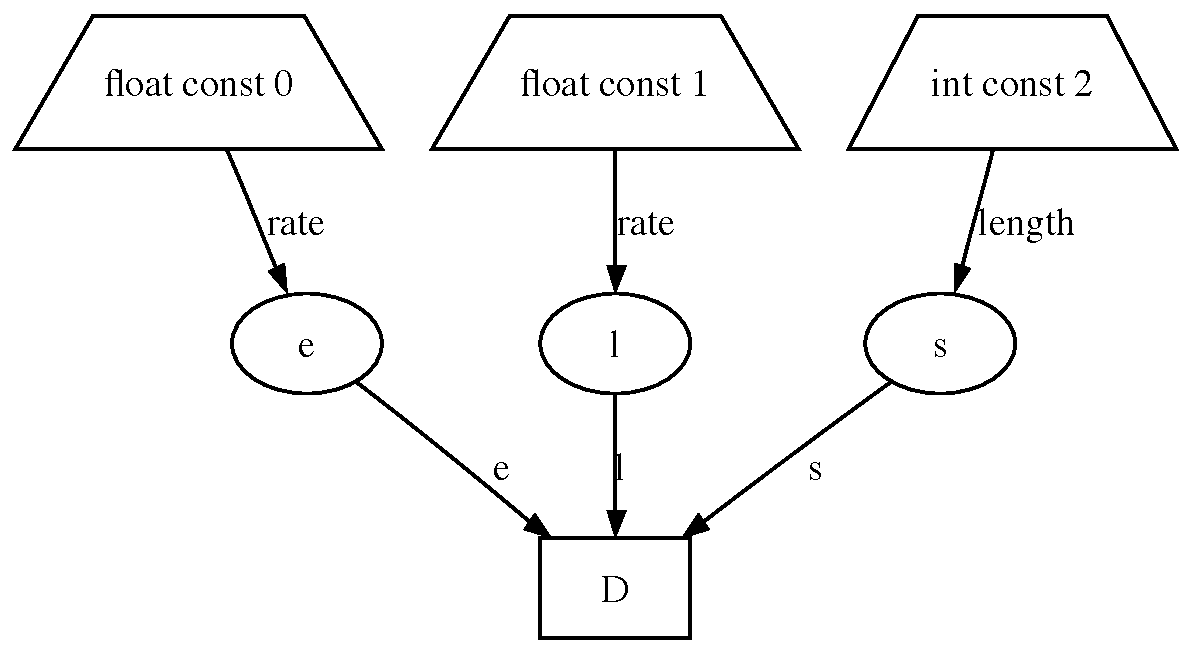
\epsfig{file=DisasterModel.pdf, width=6cm} 
\end{center} 
$D$ is shaded because it is flagged as data.

PyMC's symbol for deterministic variables is a downward-pointing triangle. A graphical representation of model \ref{disastermodel} with $r$ explicit follows:
\begin{center}
    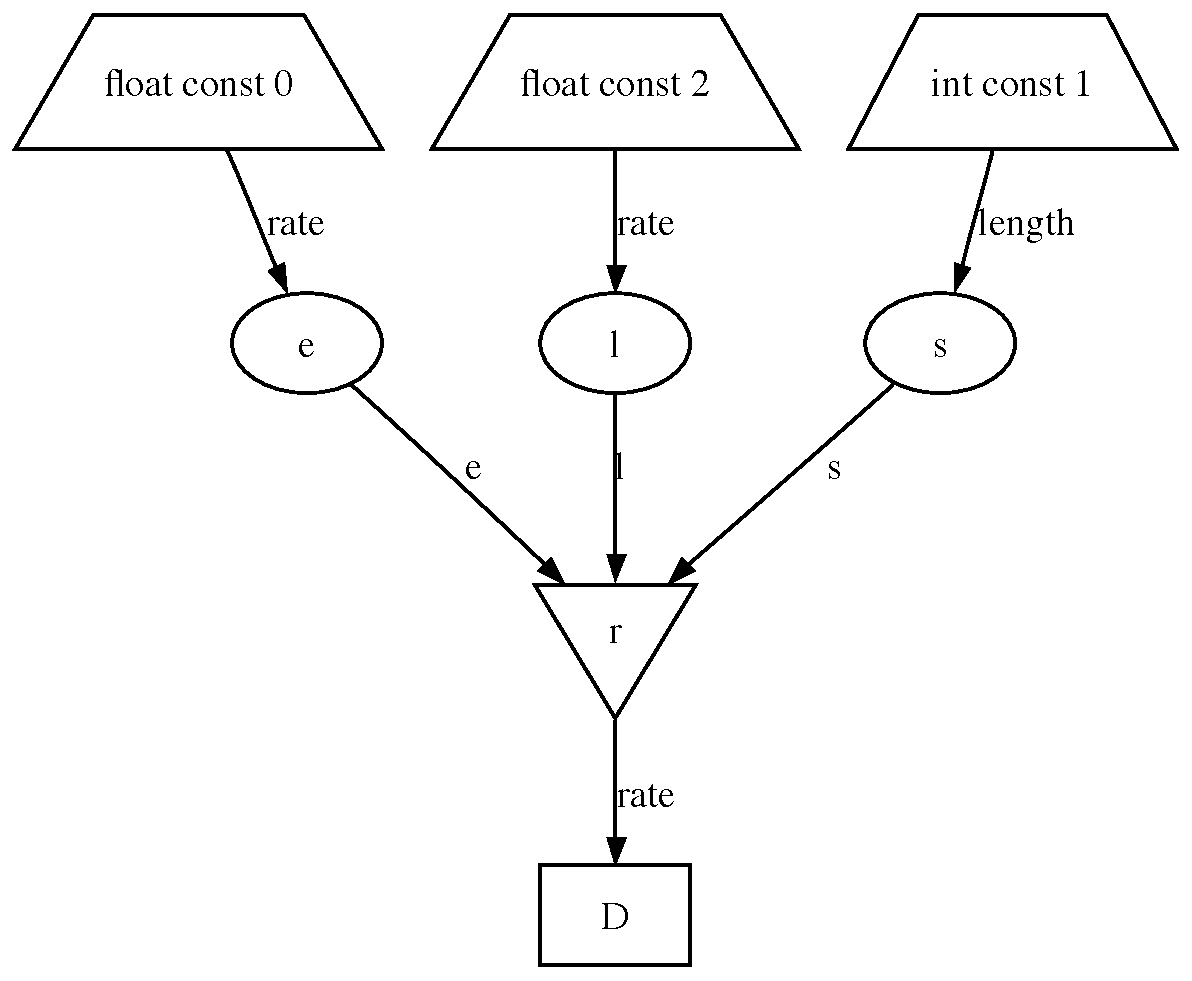
\epsfig{file=DisasterModel2.pdf, width=6cm} 
\end{center}
% Note that if a deterministic variable has more than one child, its parents each inherit all of its children when it is made implicit:
% \begin{center}
%     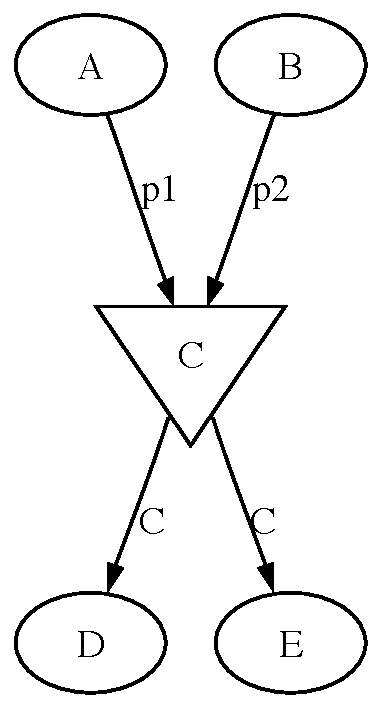
\epsfig{file=DeterministicPreInheritance.pdf, width=3.5cm} $\Rightarrow$ 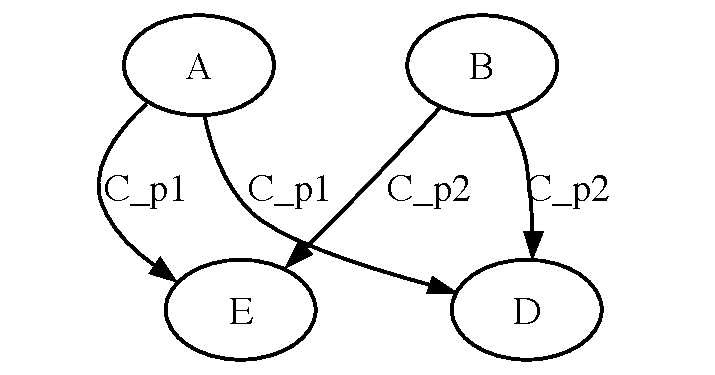
\epsfig{file=DeterministicPostInheritance.pdf, width=5cm}
% \end{center}
% These inherited children can be accessed via the \texttt{extended_children} attributes of the parents.

The symbol for factor potentials is a rectangle:
\begin{center}
    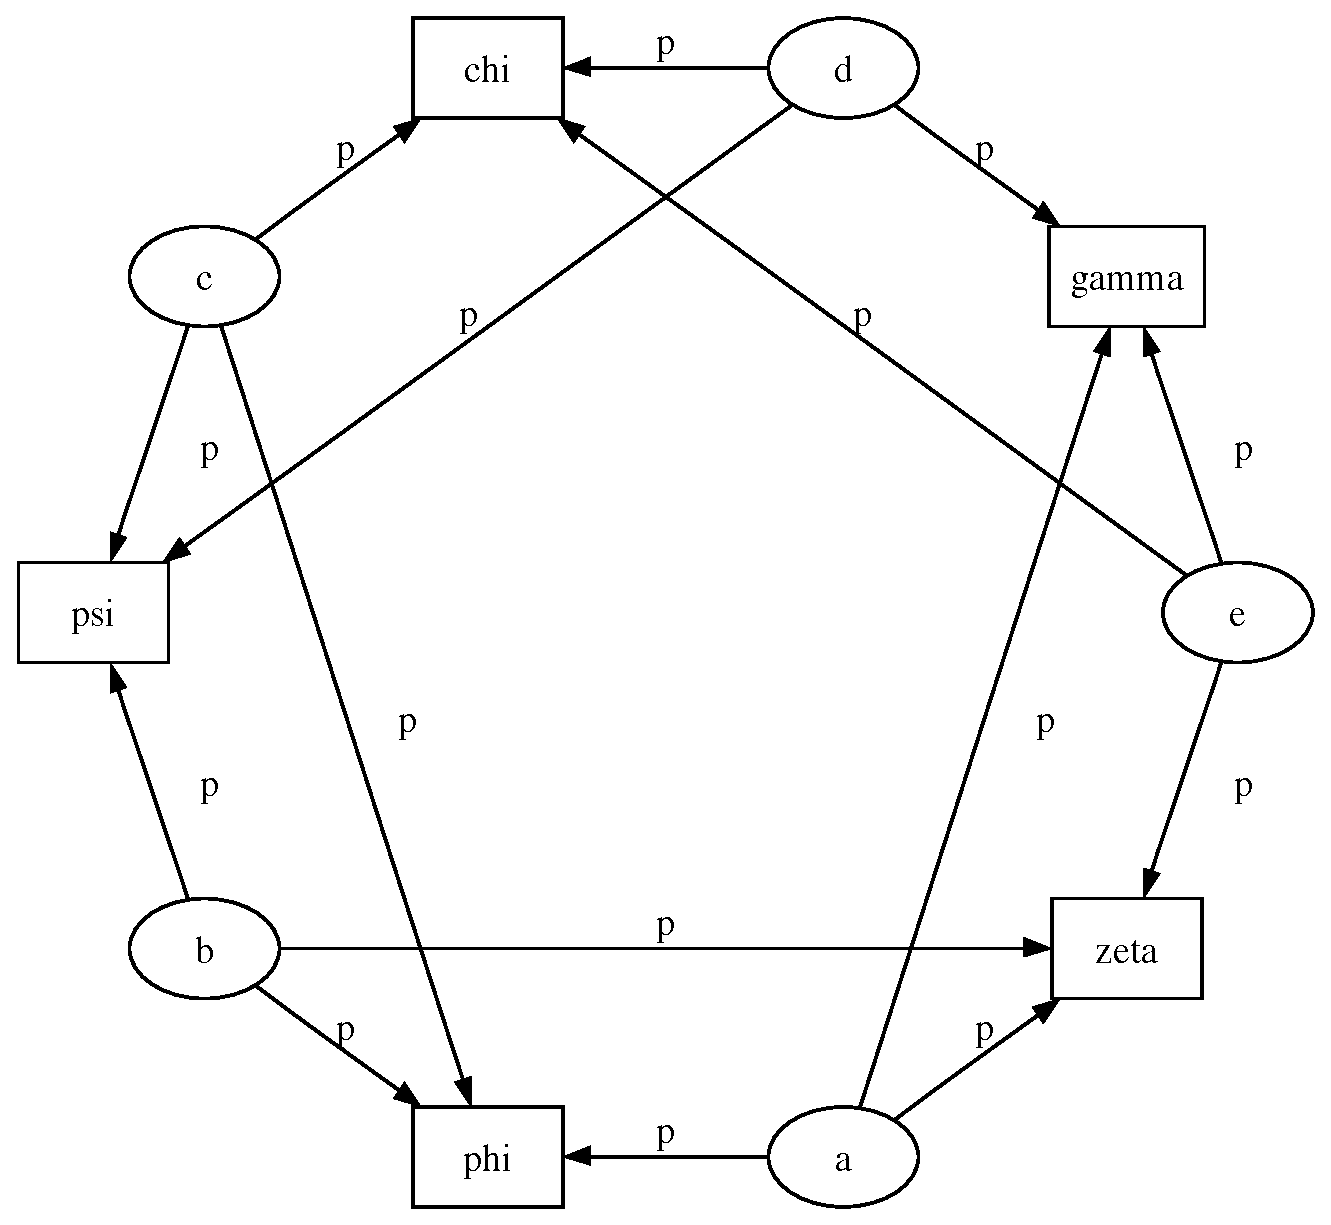
\epsfig{file=PotExample.pdf, width=10cm} 
\end{center}
Factor potentials are usually associated with \emph{undirected} grahical models. In undirected representations, each parent of a potential is connected to every other parent by an undirected edge:
\begin{center}
    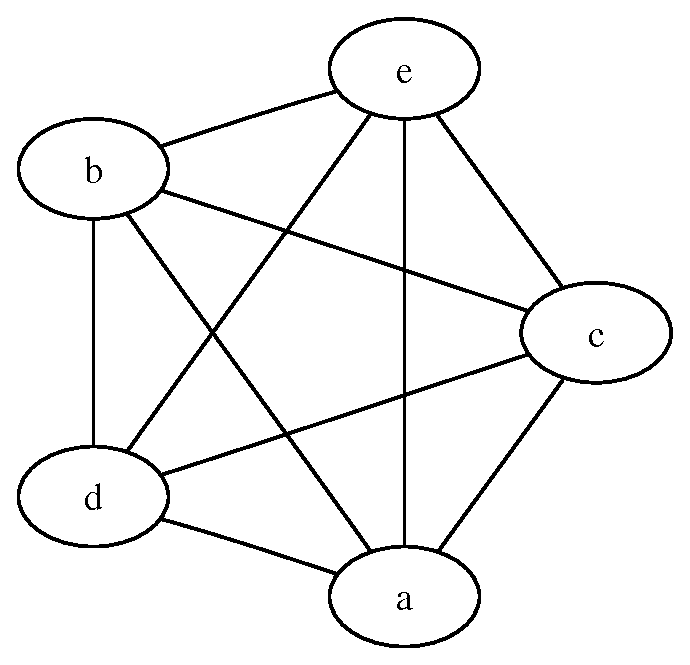
\epsfig{file=PotExampleCollapsed.pdf, width=5cm}
\end{center}

Directed or mixed graphical models can be represented in an undirected form by `moralizing', which is done by the function \texttt{moral_graph}.


\section*{Class \texttt{LazyFunction} and caching}
\label{sec:caching} 

The \texttt{logp} attributes of stochastic variables and potentials and the \texttt{value} attributes of deterministic variables are wrappers for instances of class \texttt{LazyFunction}. Lazy functions are wrappers for ordinary Python functions. A lazy function \texttt{L} could be created from a function \texttt{fun} as follows:
\begin{verbatim}
L = LazyFunction(fun, arguments)
\end{verbatim}
The argument \texttt{arguments} is a dictionary container; \texttt{fun} must accept keyword arguments only. When \texttt{L}'s \texttt{get()} method is called, the return value is the same as the call 
\begin{verbatim}
fun(**arguments.value)
\end{verbatim}
Note that no arguments need to be passed to \texttt{L.get}; lazy functions memorize their arguments.

Before calling \texttt{fun}, \texttt{L} will check the values of \texttt{arguments.variables} against an internal cache. This comparison is done \emph{by reference}, not by value, and this is part of the reason why stochastic variables' values cannot be updated in-place. If \texttt{arguments.variables}' values match a frame of the cache, the corresponding output value is returned and \texttt{fun} is not called. If a call to \texttt{fun} is needed, \texttt{arguments.variables}' values and the return value replace the oldest frame in the cache. The depth of the cache can be set using the optional init argument \texttt{cache_depth}, which defaults to 2.

Caching is helpful in MCMC, because variables' log-probabilities and values tend to be queried multiple times for the same parental value configuration. The default cache depth of 2 turns out to be most useful in Metropolis-Hastings-type algorithms involving proposed values that may be rejected.

Lazy functions are implemented in C via Pyrex.